%%%%%%%%%%%%%%%%%%%%%%%%%%%%%%%%%%%%%%%%%%%%%%%%%%%%%%%%%%%%%%%%%%%%%%%%%%%%%%%%%%%%
% Document data
%%%%%%%%%%%%%%%%%%%%%%%%%%%%%%%%%%%%%%%%%%%%%%%%%%%%%%%%%%%%%%%%%%%%%%%%%%%%%%%%%%%%
\documentclass[12pt]{article} %report allows for chapters
%%%%%%%%%%%%%%%%%%%%%%%%%%%%%%%%%%%%%%%%%%%%%%%%%%%%%%%%%%%%%%%%%%%%%%%%%%%%%%%%%%%%
\usepackage{preamble}
\usepackage{caption}
\usepackage{subcaption}

\begin{document}

\begin{center}
   \textsc{\large MATH 272, Homework 6, \emph{Solutions}}\\
\end{center}
\vspace{.5cm}

\begin{problem}
Consider the 1-dimensional wave equation given by
\[
\left(-\frac{\partial^2}{\partial x^2} +\frac{1}{c^2} \frac{\partial^2}{\partial  t^2} \right) u(x,t) = 0.
\]
We'll consider two distinct scenarios. First, we'll take an infinitely long elastic rod and second we'll take a rod of finite length with Dirichlet boundary conditions.
\begin{enumerate}[(a)]
    \item For a rod of infinite length, consider the initial conditions
    \[
    u(x,0) = \begin{cases} x+1 & -1\leq x \leq 0 \\ 1-x & 0\leq x \leq 1 \\ 0 & \textrm{otherwise} \end{cases} \qquad \textrm{and} \qquad \frac{\partial}{\partial t} u(x,0) = 0.
    \]
    Find and plot the portion of the wave that moves to the right with $c=1$.
    \item Let $u_R(x,t)$ be your solution from (a), show that this satisfies the right-moving wave equation
    \[
    \left(\frac{\partial}{\partial x} + \frac{1}{c} \frac{\partial}{\partial t} \right)u_R(x,t) = 0.
    \]
    \item Why is it that we can ignore the points where your function $u_R(x,t)$ is not differentiable even though we are considering this as a solution to a PDE?
    \item For an elastic rod $\Omega$ of finite length, $\Omega = [0,1]$, assume that we take the Dirichlet conditions $u(0,t)=0=u(1,t)$.  With the initial conditions
    \[
    u(x,0) = \sin(\pi x) \qquad \textrm{and} \qquad \frac{\partial}{\partial t} u(x,0)=0,
    \]
    find the solution using d'Alembert's formula.
    \item Let $w(x,t)$ be your solution for (d), show that it is indeed equal to
    \[
    w(x,t) = \sin(\pi x)\cos(\pi c t).
    \]
    \item With your result from (e), explain how we can decompose a standing wave into a linear combination of two waves; one moving towards the left and one moving towards the right and both reflecting off the boundary.
\end{enumerate}
\end{problem}
\begin{solution}~
\begin{enumerate}[(a)]
    \item We have that the solution is given by
\[
u(x,t) = \frac{1}{2} \left( u_L(x,t) + u_R(x,t)\right),
\]
where $u_L(x,t)$ is a portion of the wave moving to the left and $u_R(x,t)$ is the portion of the wave moving towards the right.  From our initial conditions, we have
\[
u_L(x,t) = \begin{cases} x+ct+1 & -1\leq x+ct \leq 0 \\ 1-x-ct & 0\leq x+ct \leq 1 \\ 0 & \textrm{otherwise} \end{cases} \qquad \textrm{and} \qquad u_R(x,t)=\begin{cases} x-ct+1 & -1\leq x-ct \leq 0 \\ 1-x+ct & 0\leq x-ct \leq 1 \\ 0 & \textrm{otherwise} \end{cases},
\]
which follows from d'Alembert's formula. 

We can then plot $u_R(x,t)$ for a few different times with $c=1$. 
\begin{figure}[H]
    \centering
    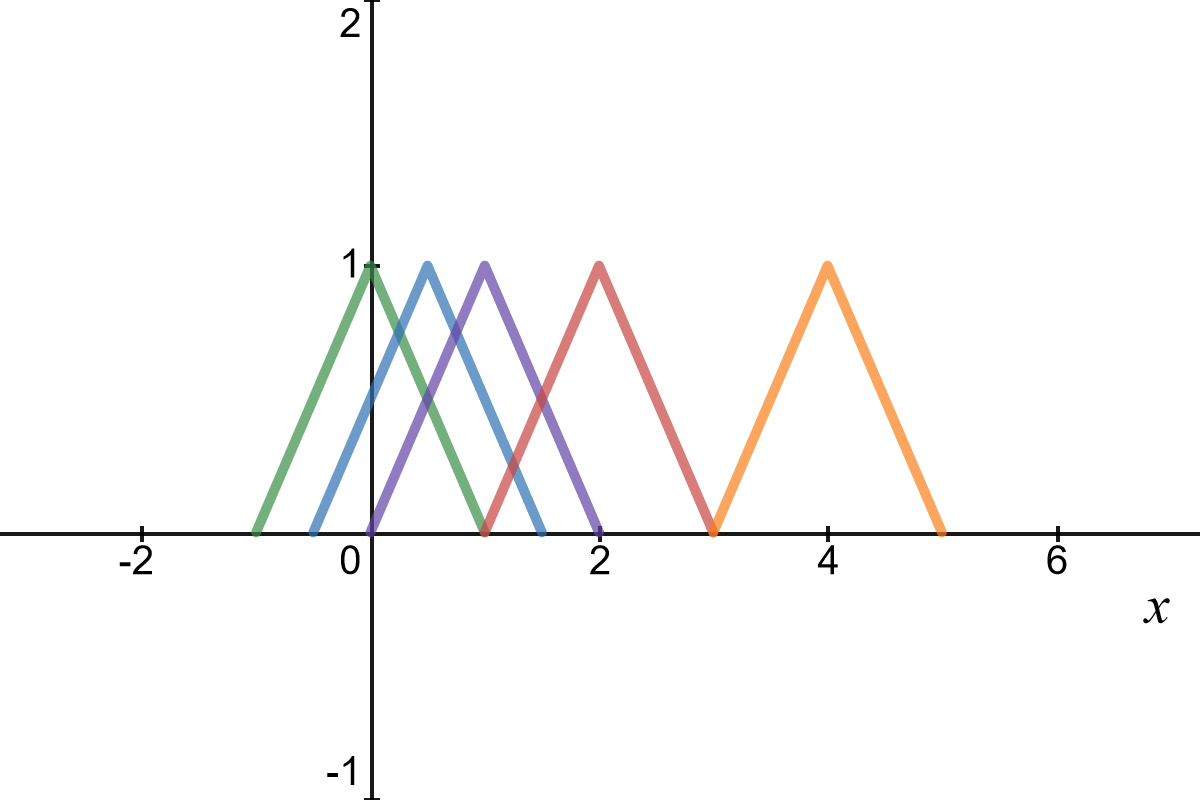
\includegraphics[width=.8\textwidth]{figures/right_moving_triangle.png}
    \caption{Plots of $u_R$ for $t=0$ (green), $t=1/2$ (blue), $t=1$ (purple), $t=2$ (red), and $t=4$ (orange).}
\end{figure}
    \item We can take the derivatives of $u_R(x,t)$ to get
    \[
    \frac{\partial}{\partial x} u_R(x,t) = \begin{cases} 1 & -1< x-ct < 0 \\ -1 & 0<x-ct < 1 \\ 0 & \textrm{otherwise} \end{cases}
    \]
    as well as
    \[
    \frac{1}{c}\frac{\partial}{\partial t} u_R(x,t) = \frac{1}{c}\begin{cases} -c & -1< x-ct < 0 \\ c & 0<x-ct < 1 \\ 0 & \textrm{otherwise} \end{cases}.
    \]
    Then, if we add the two together, we get our intended result
    \[
    \left(\frac{\partial}{\partial x} + \frac{1}{c} \frac{\partial}{\partial t} \right)u_R(x,t) = 0
    \]
    Notice, this is true aside from the three points where we see the kinks in our wave.
    
    \item The function may not be differentiable at three distinct $x$ values for every time $t$, but this is fairly unimportant.  Roughly speaking, we can choose to ignore three points in which we have issues since this works on infinitely many other points.  There is more detail here, but that is mathematics left to discover for yourself on a later day.
    
    \item From d'Alembert's formula we see that
    \[
    u_L(x,t) = \sin(\pi (x+ct)) \qquad \textrm{and} \qquad u_R(x,t) = \sin(\pi (x-ct)).
    \]
    Hence, our solution is given by
    \[
    u(x,t) = \frac{1}{2} \left(\sin(\pi (x+ct))+\sin(\pi(x-ct))\right).
    \]
    
    \item Note that we have the trigonometric identity
    \[
    \sin(a+b) = \sin(a)\cos(b)+\cos(a)\sin(b).
    \]
    Applying this to $u_L$ and $u_R$ we have
    \[
    u_L(x,t) = \sin(\pi x+\pi ct) = \sin(\pi x)\cos(\pi c t)+ \cos(\pi x)\sin(\pi c t),
    \]
    and
    \[
    u_R(x,t) = \sin(\pi x-\pi ct) = \sin(\pi x)\cos(-\pi c t)+ \cos(\pi x)\sin(-\pi c t).
    \]
    Then, we have
    \begin{align*}
        u(x,t) &= \frac{1}{2} \left(\sin(\pi x)\cos(\pi c t)+ \cos(\pi x)\sin(\pi c t) + \sin(\pi x)\cos(-\pi c t)+ \cos(\pi x)\sin(-\pi c t) \right)\\
        &= \frac{1}{2} \left( \sin(\pi x)\cos(\pi c t) + \sin(\pi x)\cos(\pi c t) + \cos(\pi x)\sin(\pi c t) - \cos(\pi x)\sin(\pi c t)\right)\\
        &= \sin(\pi x) \cos(\pi c t) = w(x,t),
    \end{align*}
    which is indeed the solution we have found to this problem previously.
    
    \item In the previous example, we took two different waves; one moving towards the left and one moving towards the right.  It turned out that adding these solutions could be cleverly combined into a single standing wave solution.  Essentially, the separation of variables seems to help us find standing waves (though it can also find traveling waves) where as the d'Alembert method decomposes waves into their portions that move in either direction naturally. 
    
    In this case, it must be that the traveling waves are reflected by the boundaries in order to produce a standing wave.  If you play with a slinky, you may be able to discover this behavior yourself!
  \end{enumerate}
\end{solution}

\begin{problem}
    Consider the 1-dimensional wave equation given by
    \[
    \left( - \frac{\partial^2}{\partial x^2} +\frac{1}{c^2} \frac{\partial^2}{\partial t^2} \right) u(x,t) =0,
    \]
    with the domain $\Omega$ as the unit interval on the $x$-axis.  We shall fix the string at each endpoint which requires $u(0,t)=0$ and $u(1,t)=0$ for all $t$.  Take the initial condition as well to be a plucked string so that $u(x,0)=\sin(\pi x)$ and $\frac{\partial}{\partial t}u(x,0)=0$. 
    \begin{enumerate}[(a)]
        \item Use the separation of variables ansatz $u(x,t)=X(x)T(t)$ to get a new separation constant. This will give two ODEs: one will be in terms of $X(x)$ and the other will be in terms of $T(t)$.
        \item Use the boundary conditions and solve the ODE that is in terms of $X(x)$ which will simultaneously find the allowed values for the separation constant.
        \item Using these allowed values for the separation constant, find the solution for $T(t)$.
        \item Find the particular solution for $u(x,t)$ by matching the initial condition.
        \item Plot your solution for $x\in [0,1]$ and $t\in [0,\infty)$ (i.e., just plot up to a large value of $t$). In this case, compare your plots for $c=1/2$ and $c=1$.
    \end{enumerate}
\end{problem}
\begin{solution}~
\begin{enumerate}[(a)]
    \item If we take $u(x,t)=X(x)T(t)$, then plugging this into the PDE yields
    \[
    -X''T+\frac{1}{c^2} XT'' = 0.
    \]
    We can then isolate each variable on one side of the equal sign to get
    \[
    \frac{X''}{X} = \frac{1}{c^2}\frac{T''}{T}.
    \]
    Note that the left hand side depends only on $x$, whereas the right hand side depends solely on $t$. Thus, it must be that both sides equal the same constant $\lambda$. This gives us two ODEs
    \[
    X'' -\lambda X = 0 \qquad \textrm{and} \qquad T'' -c^2 \lambda T = 0.
    \]
    
    \item The boundary conditions are a spatial condition and thus we must satisfy them independent of time.  Hence, we must have that $X(0)=0$ and $X(1)=0$ so that $u(0,t)=0$ and $u(1,t)=0$ respectively.  This means that $\lambda<0$ so that we get
    \[
    X(x) = a\cos(\sqrt{-\lambda}x) +b \sin(\sqrt{-\lambda} x),
    \]
    since if $\lambda \geq 0$ we will only get constant solutions which are trivial and can't match the initial conditions or exponential solutions which can't match the boundary conditions.  Applying the boundary conditions yields that $A=0$ and $\sqrt{-\lambda}=n\pi$ for any positive integer $n$. Thus we have
    \[
    X_n(x) = a_n \sin(n\pi x), 
    \]
    is (nontrivial) a solution to this ODE for every positive integer $n$.
    
    \item Using this result for $\lambda$, we have that
    \[
    T_n(t) = b_n \sin(cn\pi t)+c_n \cos(cn\pi t),
    \]
    for every positive integer $n$.  
    
    \item Combining to get $u_n(x,t) =X_n(x)T_n(t)$, we can write
    \[
    u_n(x,t) = \left(a_n \sin(cn\pi t)+b_n \cos(cn\pi t)\right) \sin(n\pi x),
    \]
    is a general solution for each positive integer $n$.  Note that we have just renamed constants here to write this more simply.  Now, in general, a sum of these solutions is also a solution, but we have
    \[
    u(x,0)=\sin(\pi x),
    \]
    which means that $n=1$, $a_1=0$, and $b_1=1$.  All other constants $a_j$ and $b_j$ are all zero.  One can then check that our solution
    \[
    u(x,t) = \cos(c \pi t) \sin(\pi x),
    \]
    satisfies $\frac{\partial}{\partial t} u(x,0) = 0$.  
    
    \item Here are the plots for these functions. Note that in this case, we plotted the solution as a surface with one of the axes representing time.  This still just shows how the 1-dimensional elastic evolves over time. We see that when $c$ is increased, the elastic vibrates more quickly.
    
                \begin{figure}[H]
                	\centering
                	\def\svgwidth{0.6\columnwidth}
                	\input{figures/wave_solution_c=1_2.pdf_tex}
                    \caption{The graph of the solution $u(x,t)$ for $c=1/2$.}
                \end{figure}
                \begin{figure}[H]
                                	\centering
                                	\def\svgwidth{0.6\columnwidth}
                                	\input{figures/wave_solution_c=1.pdf_tex}
                                    \caption{The graph of the solution $u(x,t)$ for $c=1$.}
                                \end{figure}
\end{enumerate}
\end{solution}



\begin{problem}
Consider the heat flow problem on the region $\Omega=[0,1]$ given by
\[
\begin{cases}
\frac{\partial}{\partial t} u(x,t) = \frac{\partial^2}{\partial x^2} u(x,t) - 1, & \textrm{in $(0,1)$},\\
u(0,t)=0 \textrm{~and~} u(1,t)=1, & \text{as boundary conditions},\\
u(x,0) = \sin\left(\pi x\right) + \frac{1}{2}(x^2+x), & \textrm{as the initial condition}.
\end{cases}
\]
This corresponds to a rod kept at fixed temperatures at the endpoints that starts with a warm center initially.
\begin{enumerate}[(a)]
    \item As with the previous homework, take an ansatz
    \[
    u(x,t) = v(x,t) + u_E(x)
    \]
    where $v(x,t)$ solves the following problem
    \[
\begin{cases}
\frac{\partial}{\partial t} v(x,t) = \frac{\partial^2}{\partial x^2} v(x,t), & \textrm{in $(0,1)$},\\
v(0,t)=0 \textrm{~and~} v(1,t)=0, & \text{as boundary conditions}.
\end{cases}
    \]
    Find the general solution $v(x,t)$ using separation of variables. \emph{Hint: feel free to use the work in the notes (Example ``Solving the Heat Equation" and Example ``Particular Solution to the 1D Heat Equation").}

    \item Show that for $u(x,t)$ to be a solution that
    \[
    \frac{\partial^2}{\partial x^2} u_E(x) = 1.
    \]

    \item Find the solution $u_E(x)$ to the following problem
    \[
    \begin{cases}
    \frac{\partial^2}{\partial x^2} u_E(x) = 1, & \textrm{in $(0,1)$},\\
    u_E(0)=0 \textrm{~and~} u_E(1)=1, & \text{as boundary conditions}.
    \end{cases}
    \]
    
    \item All is left in determining the function $u(x,t)$ is to determine the particular solution that satisfies the initial condition. Using our ansatz $u(x,t)=v(x,t)+u_E(x)$, determine the particular solution.
\end{enumerate}
\end{problem}
\begin{solution}~
    \begin{enumerate}[(a)]
    \item Based on the examples, we know
    \[
    v(x,t) = Ae^{-\lambda t} \sin(\sqrt{\lambda}x)+B e^{-\lambda t} \cos(\sqrt{\lambda}x).
    \]
    Taking the boundary conditions $v(0,t)=0$ yields that $B=0$ as in the example and taking $v(1,t)=0$ makes us realize $\sqrt{\lambda} = n\pi$ for any integer $n$ (again via the examples). Hence, 
    \[
    v(x,t) = A_n e^{-n^2 \pi^2 t} \sin(n\pi x).
    \]

    \item If we apply our ansatz with our given information about $v(x,t)$ we must have
    \begin{align*}
    -\frac{\partial}{\partial t}u(x,t) &= \frac{\partial^2}{\partial x^2}u(x,t)-1\\
     -\frac{\partial}{\partial t}(v(x,t)+u_E(x)) &= \frac{\partial^2}{\partial x^2}(v(x,t)+u_E(x))-1\\
    0 &= \frac{\partial^2}{\partial x^2}u_E(x)-1,
    \end{align*}
    since $v(x,t)$ is a solution to the heat equation. Thus,
    \[
    \frac{\partial^2}{\partial x^2}u_E(x)=1
    \]

    \item To find this particular solution, we first note that the general solution can be found by integrating twice. That is,
    \[
    u_E(x) = \frac{1}{2}x^2+c_1x+c_2.
    \]
    Applying the boundary conditions,
    \[
    0=u_E(0)=c_2,
    \]
    so $c_2=0$ and
    \[
    1=u_E(1)=\frac{1}{2}+c_1,
    \]
    so $c_1=\frac{1}{2}$. Thus,
    \[
    u_E(x)=\frac{1}{2}(x^2+x).
    \]

    \item To find our particular solution, we require
    \[
    u(x,0) = v(x,0)+u_E(x),
    \]
    which means
    \[
    \sin\left(\pi x\right) + \frac{1}{2}(x^2+x)= A_n \sin(n\pi x) + \frac{1}{2}(x^2+x),
    \]
    and we find that $n=1$ and $A_n=1$ as well. Hence, our particular solution is
    \[
    u(x,t) = v(x,t)+u_E(x) = e^{-\pi^2 t}\sin\left(\pi x\right) + \frac{1}{2}(x^2+x).
    \]
\end{enumerate}
\end{solution}

\begin{problem}[Bonus]
Take the set up from the previous problem, but let us modify the initial conditions and boundary conditions slightly. Instead, we have
\[
\begin{cases}
\frac{\partial}{\partial t} u(x,t) = \frac{\partial^2}{\partial x^2} u(x,t) - 1, & \textrm{in $(0,1)$},\\
u(0,t)=0 \textrm{~and~} u(1,t)=0, & \text{as boundary conditions},\\
u(x,0) = -(2x-1)^2+1, & \textrm{as the initial condition}.
\end{cases}
\]
We want to discover how we can possibly solve problems with more general initial conditions. If you pay attention to the work in 3, you will find the initial conditions were chosen in a very contrived manner. This is not ideal if we want to solve a problem in general!

Taking a look at Example ``Particular Solution to the 1D Heat Equation" in the notes. Notice that it is of the form
\[
u_n(x,t) = A_ne^{-n^2\pi^2 t} \sin(n \pi x),
\]
is a general solution for all integers $n$. 
\begin{enumerate}[(a)]
    \item Can you recreate the initial condition $u(x,0)$ with a single $u_n(x,0)$?
    \item Can you recreate the initial condition with a finite sum of $u_n(x,0)$?
    \item Suppose that we can take an infinite sum
    \[
    \sum_{n=1}^\infty A_n e^{-n^2\pi^2} \sin(n \pi x).
    \]
    Show that
    \[
    \sum_{n=1}^\infty -\frac{8\left(2\left(-1\right)^{n}-2\right)}{\pi^{3}n^{3}}\sin\left(n\pi x\right) = u(x,0)
    \]
    by plotting both $u(x,0)$ and the sum (up to a large $N$) simultaneously. It is worthwhile to steadily increase the upper bound of the sum to see this convergence!
    \item Comment on this. Do you think this is something we can do in general for any initial condition?
\end{enumerate}
\end{problem}

\begin{solution}
\begin{enumerate}[(a)]
    \item No! There is no way that we can have any kind of sine function equal to a polynomial. Just look at the Taylor series for $\sin(x)$!
    \item No, this is also not doable. Once again, you'd have an infinite polynomial via the Taylor series. This cannot be.
    \item Here is the figure.
    \begin{figure}[H]
\centering
    \begin{subfigure}[b]{0.3\textwidth}
        \centering
        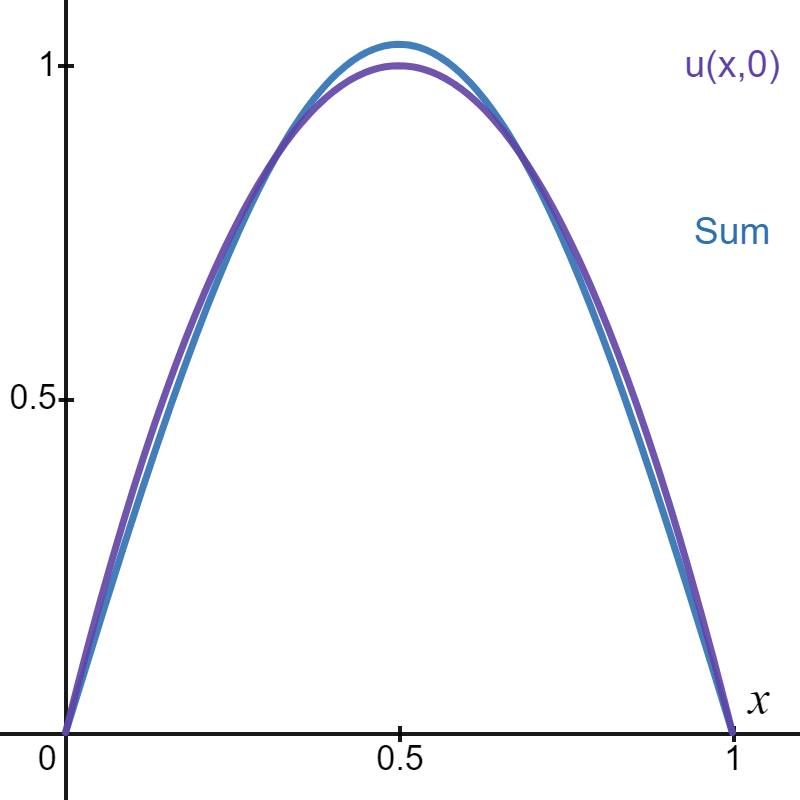
\includegraphics[width=\textwidth]{figures/sum_n1.png}
        \caption{Plotting both $u(x,0)$ and the sum up to $N=1$.}
    \end{subfigure}
    \hfill
    \begin{subfigure}[b]{0.3\textwidth}
        \centering
        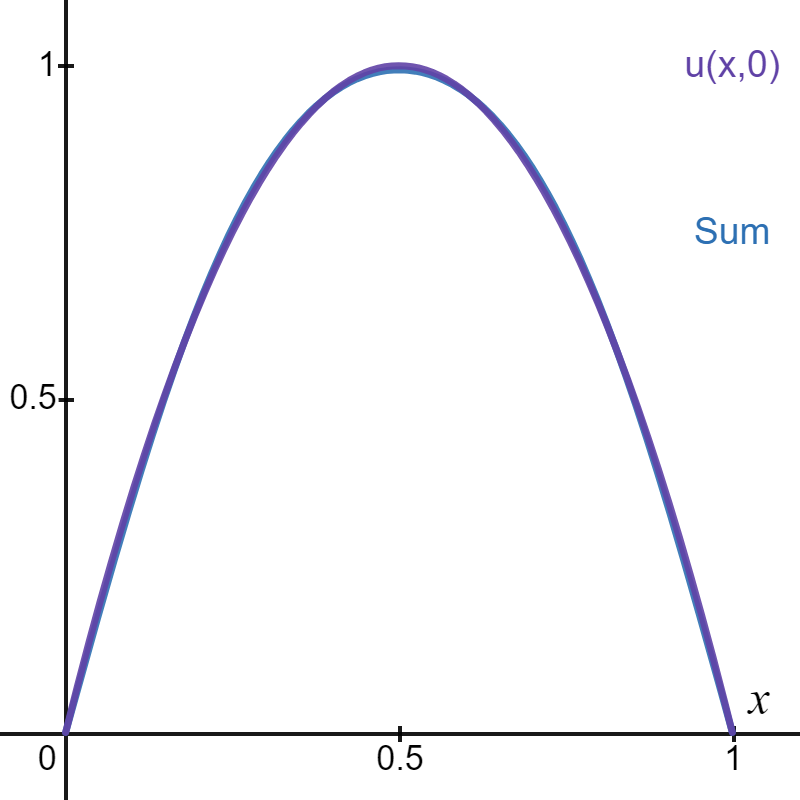
\includegraphics[width=\textwidth]{figures/sum_n4.png}
        \caption{Plotting both $u(x,0)$ and the sum up to $N=4$.}
    \end{subfigure}
    \hfill
    \begin{subfigure}[b]{0.3\textwidth}
        \centering
        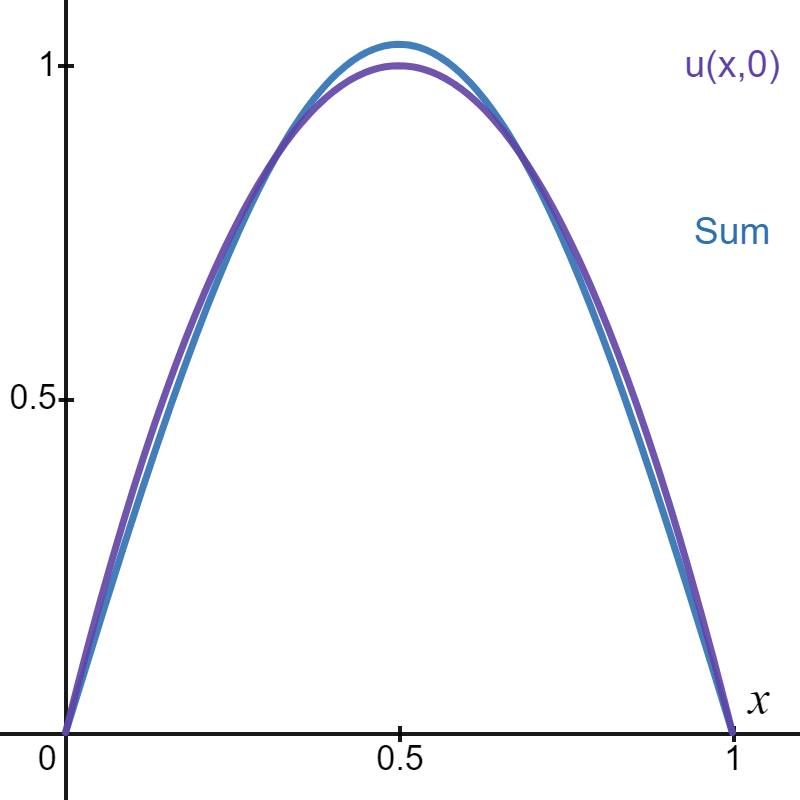
\includegraphics[width=\textwidth]{figures/sum_n1.png}
        \caption{Plotting both $u(x,0)$ and the sum up to $N=50$.}
    \end{subfigure}
    \end{figure}
\end{enumerate}
\end{solution}
\end{document}

\end{document}